\PassOptionsToPackage{unicode=true}{hyperref} % options for packages loaded elsewhere
\PassOptionsToPackage{hyphens}{url}
%
\documentclass[10pt,ignorenonframetext,]{beamer}
\setbeamertemplate{caption}[numbered]
\setbeamertemplate{caption label separator}{: }
\setbeamercolor{caption name}{fg=normal text.fg}
\beamertemplatenavigationsymbolsempty
\usepackage{lmodern}
\usepackage{amssymb,amsmath}
\usepackage{ifxetex,ifluatex}
\usepackage{fixltx2e} % provides \textsubscript
\ifnum 0\ifxetex 1\fi\ifluatex 1\fi=0 % if pdftex
  \usepackage[T1]{fontenc}
  \usepackage[utf8]{inputenc}
  \usepackage{textcomp} % provides euro and other symbols
\else % if luatex or xelatex
  \usepackage{unicode-math}
  \defaultfontfeatures{Ligatures=TeX,Scale=MatchLowercase}
\fi
% use upquote if available, for straight quotes in verbatim environments
\IfFileExists{upquote.sty}{\usepackage{upquote}}{}
% use microtype if available
\IfFileExists{microtype.sty}{%
\usepackage[]{microtype}
\UseMicrotypeSet[protrusion]{basicmath} % disable protrusion for tt fonts
}{}
\IfFileExists{parskip.sty}{%
\usepackage{parskip}
}{% else
\setlength{\parindent}{0pt}
\setlength{\parskip}{6pt plus 2pt minus 1pt}
}
\usepackage{hyperref}
\hypersetup{
            pdftitle={Noisy Gradient-Descent Bit Flipping (NGDBF) Decoding Algorithm},
            pdfauthor={Eric Reiss},
            pdfborder={0 0 0},
            breaklinks=true}
\urlstyle{same}  % don't use monospace font for urls
\newif\ifbibliography
\usepackage{graphicx,grffile}
\makeatletter
\def\maxwidth{\ifdim\Gin@nat@width>\linewidth\linewidth\else\Gin@nat@width\fi}
\def\maxheight{\ifdim\Gin@nat@height>\textheight\textheight\else\Gin@nat@height\fi}
\makeatother
% Scale images if necessary, so that they will not overflow the page
% margins by default, and it is still possible to overwrite the defaults
% using explicit options in \includegraphics[width, height, ...]{}
\setkeys{Gin}{width=\maxwidth,height=\maxheight,keepaspectratio}
% Prevent slide breaks in the middle of a paragraph:
\widowpenalties 1 10000
\raggedbottom
\setbeamertemplate{part page}{
\centering
\begin{beamercolorbox}[sep=16pt,center]{part title}
  \usebeamerfont{part title}\insertpart\par
\end{beamercolorbox}
}
\setbeamertemplate{section page}{
\centering
\begin{beamercolorbox}[sep=12pt,center]{part title}
  \usebeamerfont{section title}\insertsection\par
\end{beamercolorbox}
}
\setbeamertemplate{subsection page}{
\centering
\begin{beamercolorbox}[sep=8pt,center]{part title}
  \usebeamerfont{subsection title}\insertsubsection\par
\end{beamercolorbox}
}
\AtBeginPart{
  \frame{\partpage}
}
\AtBeginSection{
  \ifbibliography
  \else
    \frame{\sectionpage}
  \fi
}
\AtBeginSubsection{
  \frame{\subsectionpage}
}
\setlength{\emergencystretch}{3em}  % prevent overfull lines
\providecommand{\tightlist}{%
  \setlength{\itemsep}{0pt}\setlength{\parskip}{0pt}}
\setcounter{secnumdepth}{0}

% set default figure placement to htbp
\makeatletter
\def\fps@figure{htbp}
\makeatother


\title{Noisy Gradient-Descent Bit Flipping (NGDBF) Decoding Algorithm}
\providecommand{\subtitle}[1]{}
\subtitle{A probabilistic decoding algorithm}
\author{Eric Reiss}
\date{}


\usepackage[most]{tcolorbox}

\tcbset{
  frame code={},
  center title,
  left=0pt,
  right=0pt,
  top=0pt,
  bottom=0pt,
  colback=blue!20,
  colframe=white,
  width=\dimexpr\textwidth\relax,
  enlarge left by=0mm,
  boxsep=5pt,
  arc=0pt,outer arc=0pt,
}



\setbeamertemplate{title page}{

  \begin{picture}(0,0)
    
     
    \put(0,-40.7){%
      \begin{minipage}[b][45mm][t]{226mm}
        \usebeamerfont{title}{\inserttitle\par}
        \usebeamerfont{subtitle}{\insertsubtitle\par}
        \vspace{0.5cm}
        \usebeamerfont{author}{\insertauthor\par}
        \usebeamerfont{author}{Utah State University\par}
      \end{minipage}
    }
    
  \end{picture}
}


\setbeamertemplate{itemize/enumerate subbody begin}{\vspace{0.125cm}\begin{tcolorbox}[colback=red!20]}
\setbeamertemplate{itemize/enumerate subbody end}{\end{tcolorbox}\vspace{0.125cm}}
\setbeamertemplate{itemize/enumerate body begin}{\vspace{0.125cm}\begin{tcolorbox}}
\setbeamertemplate{itemize/enumerate body end}{\end{tcolorbox}\vspace{0.125cm}}
\setbeamertemplate{itemize/enumerate item end}{\vspace{0.125cm}}

\setlength{\itemsep}{0.5cm}

\makeatletter
\addtobeamertemplate{itemize begin}{
\def\@listi{\leftmargin\leftmargini
              \topsep    0pt
              \parsep    0pt
              \itemsep   3pt plus 2pt minus 3pt}
\partopsep 0pt
}
\makeatother



\begin{document}
\frame{\titlepage}

\begin{frame}{Making slides}
\protect\hypertarget{making-slides}{}
\begin{itemize}[<+->]
\item
  I like HTML presentations based on
  \href{https://www.w3.org/Talks/Tools/Slidy2/Overview.html}{Slidy}, but
  many prefer PDF slides produced by
  \href{https://www.ctan.org/pkg/beamer}{\LaTeX/Beamer}.
\item
  It can be a challenge to write code in either HTML or \LaTeX.
\item
  \href{}{Markdown and Pandoc} provide an easy text-based syntax for
  writing papers and presentations.\\
\item
  This template is designed to work with Pandoc to simultaneously:

  \begin{itemize}[<+->]
  \tightlist
  \item
    Produce html output based on slidy
  \item
    Produce matching PDF output based on \LaTeX/Beamer
  \end{itemize}
\end{itemize}
\end{frame}

\begin{frame}[fragile]{Procedure}
\protect\hypertarget{procedure}{}
\begin{enumerate}[<+->]
\tightlist
\item
  Prepare slides in a text document using Markdown syntax.
\item
  Place any images in the \texttt{figures/} subdirectory.
\item
  Edit the included \texttt{Makefile} to specify the presentation name
  and other details.
\item
  Build the presentation by running \texttt{make}
\end{enumerate}
\end{frame}

\begin{frame}[fragile]{Including Figures}
\protect\hypertarget{including-figures}{}
To include a figure using Markdown, use this syntax:

\begin{verbatim}
![Optional figure caption.](figures/example.png){width=60%}
\end{verbatim}

Result:

\begin{figure}
\centering
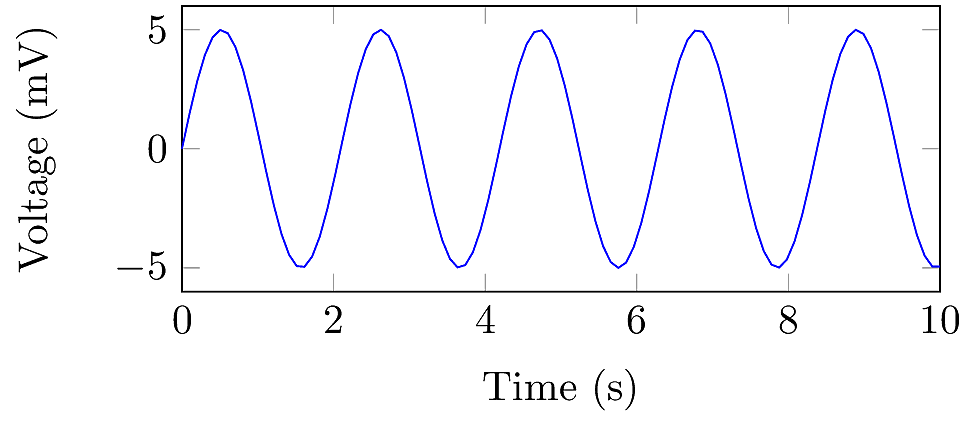
\includegraphics[width=0.6\textwidth,height=\textheight]{figures/example.png}
\caption{Optional figure caption.}
\end{figure}
\end{frame}

\begin{frame}{Two-Column Slides}
\protect\hypertarget{two-column-slides}{}
Starting two-column mode:

Here is a column.

\begin{itemize}[<+->]
\tightlist
\item
  Text.
\item
  More text.
\item
  Description.
\item
  Discussion.
\end{itemize}

And another column.

\begin{figure}
\centering
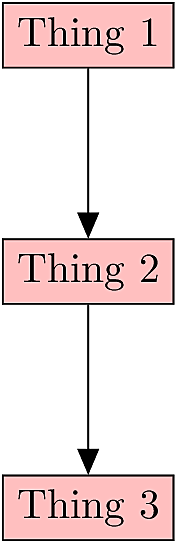
\includegraphics[width=0.2\textwidth,height=\textheight]{figures/tall_figure.png}
\caption{A tall figure.}
\end{figure}

Columns are now over.
\end{frame}

\begin{frame}{Two-Column Slides}
\protect\hypertarget{two-column-slides-1}{}
Starting two-column mode:

\begin{columns}[T]
\begin{column}{0.4\textwidth}
Here is a column.

\begin{itemize}[<+->]
\tightlist
\item
  Text.
\item
  More text.
\item
  Description.
\item
  Discussion.
\end{itemize}
\end{column}

\begin{column}{0.4\textwidth}
And another column.

\begin{figure}
\centering
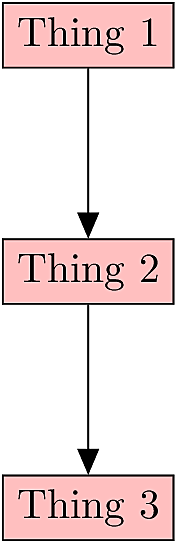
\includegraphics[width=0.2\textwidth,height=\textheight]{figures/tall_figure.png}
\caption{A tall figure.}
\end{figure}
\end{column}
\end{columns}

Columns are now over.
\end{frame}

\end{document}
